\documentclass[a4paper,14pt]{article}
\usepackage{float}
\usepackage{extsizes}
\usepackage{amsmath}
\usepackage{amssymb}
\everymath{\displaystyle}
\usepackage{geometry}
\usepackage{fancyhdr}
\usepackage{multicol}
\usepackage{graphicx}
\usepackage[brazil]{babel}
\usepackage[shortlabels]{enumitem}
\usepackage{cancel}
\columnsep=2cm
\hoffset=0cm
\textwidth=8cm
\setlength{\columnseprule}{.1pt}
\setlength{\columnsep}{2cm}
\renewcommand{\headrulewidth}{0pt}
\geometry{top=1in, bottom=1in, left=0.7in, right=0.5in}

\pagestyle{fancy}
\fancyhf{}
\fancyfoot[C]{\thepage}

\begin{document}
	
	\noindent\textbf{8FMA37~Matemática} 
	
	\begin{center}Problemas com dois móveis (II) (Versão estudante)
	\end{center}
	
	\noindent\textbf{Nome:} \underline{\hspace{10cm}}
	\noindent\textbf{Data:} \underline{\hspace{4cm}}
	
	%\section*{Questões de Matemática}
	
    \begin{multicols}{2}
    	\begin{enumerate}
    		\item Ana e Cecília fazem uma competição de remo para ver quem percorre mais rápido um trecho de um rio de 1,5 km de extensão. Ana parte de uma extremidade às 9h, e Cecília parte da outra extremidade às 09h20min. Às 10h10min, ambas se encontram exatamente no meio do trecho.
    		\begin{enumerate}[a)]
    			\item Quem ganhou a aposta? \\\\\\\\\\\\\\\\\\\\\\
    			\item Qual foi o tempo de vantagem da vencedora? \\\\\\\\\\\\\\\\\\\\\\
    		\end{enumerate}
    	    \item Um avião parte da Bélgica em direção a São Paulo voando a 723 km/h, 4 horas depois, outro avião parte de São Paulo em direção à Bélgica, a uma velocidade de 402 km/h. Os aviões cruzam-se a uma distância de 2412 km de São Paulo. Qual é a distância de São Paulo à Bélgica? \\\\\\\\\\\\\\
    	    \item Um carro saiu de Marília em direção a São Paulo, mantendo velocidade constante; outro carro havia saído 3 horas antes de São Paulo, a uma velocidade igual a $\frac{2}{5}$ da velocidade do primeiro carro. Os carros encontram-se exatamente na metade do percurso. Quanto tempo durou a viagem do carro mais rápido? \\\\\\\\\\\\\\\\
    	    \item Numa competição, duas jangadas partem de dois pontos diferentes, $A$ e $B$, de um lago. A primeira jangada parte de $A$ em direção a $B$ exatamente às 08h10min; a segunda jangada parte de $B$ em direção a $A$ às 08h35min. A segunda jangada desenvolve 6 km/h e cruza com a primeira jangada às 10h50min, a 12 km do ponto $A$.
    	    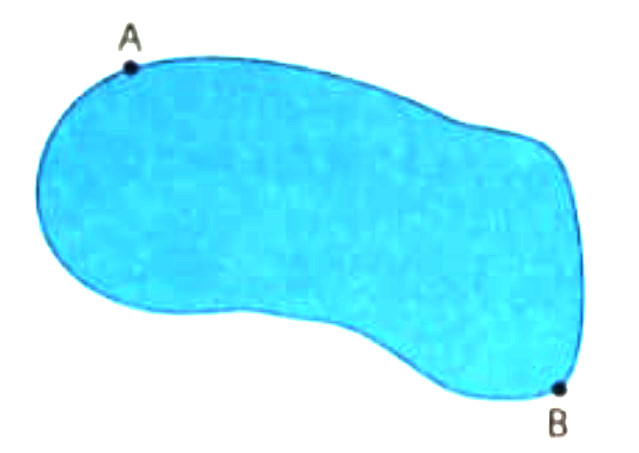
\includegraphics[width=1\linewidth]{8FMA37_imagens/imagem1}
    	    
    	    \begin{enumerate}[a)]
    	    	\item Qual é a velocidade da primeira jangada? \\\\\\\\\\\\\\\\
    	    	\item Qual é a distância entre os pontos $A$ e $B$? \\\\\\\\\\\\\\\\
    	    \end{enumerate}
            \item Um trem de passageiros parte da cidade $A$ e viaja em direção à cidade $B$, mantendo uma velocidade média de 80 km/h. Duas horas antes, havia partido da cidade $B$ um trem de carga para a cidade $A$, desenvolvendo uma velocidade média igual a $\frac{4}{5}$ da velocidade do trem de passageiros. Os dois trens encontram-se numa cidade a 400 km da cidade $B$. Qual é o comprimento da linha entre essas cidades? \\\\\\\\\\\\\\\\\\
            \item Às 8h parte uma barca da ilha $A$ em direção ao porto $B$, desenvolvendo uma velocidade de 25 km/h; às 08h21min parte de $B$, com destino a $A$, uma barca 15 km/h mais veloz. As duas barcas cruzam-se às 09h21min. Qual é a distância entre a ilha e o porto? \\\\\\\\\\\\\\\\\\\\
            \item Dois teleféricos levam ao topo de uma montanha. Um deles parte às 10h e sobe com velocidade de 3 m/s; ao chegar, fica parado durante 5 min e desce com velocidade de 5 m/s; o outro parte às 10h25min e sobe com velocidade de 4,5 m/s, cruzando com o primeiro, que descia, às 10h55min. Quantos metros tem o percurso de subida(ou descida) dos teleféricos? \\\\\\\\\\\\\\\\\\\\\\\\\\\\\\\\\\\\\\\\\\\\\\\\\\\\\\\\\\
            \item Maurício foi de carro de Bauru a Campinas em 4 horas. Suzana saiu de Bauru ao mesmo tempo, mas dirigiu uma velocidade 15 km/h maior e chegou a Campinas 45 minutos antes de Maurício. A distância de Bauru a Campinas, em quilômetros, é:
            \begin{enumerate}[a)]
            	\item 260
            	\item 205
            	\item 190
            	\item 175
            	\item 130
            \end{enumerate}
    	\end{enumerate}
    $~$ \\ $~$ \\ $~$ \\ $~$ \\ $~$ \\ $~$ \\ $~$ \\ $~$ \\ $~$ \\ $~$ \\ $~$ \\ $~$ \\ $~$ \\ $~$ \\ $~$ \\ $~$ \\ $~$ \\ $~$ \\ $~$ \\ $~$ \\ $~$ \\ $~$ \\ $~$ \\ $~$ \\ $~$ \\ $~$
    \end{multicols}
\end{document}